\FloatBarrier

\section{Beyond-OCEAN Persona Adapters}\label{sec:appendix-beyond-ocean}

% Data (sycophancy) [PUBLIC]: persona-cartography/monorepo @ fine_tuning/llama-3.1-8b-it/other/sycophancy/{amplifier,suppressor}/vsyco1_paired_dpo/evals/{mcq/{sycophancy_sweep,mmlu},coconot}/
% Data (psychopathy) [GATED, access on request]: persona-cartography/psychopathy-persona-adapters-llama-3.1-8b @ fine_tuning/llama-3.1-8b-it/other/psychopathy/{amplifier,suppressor}/vpsyc1_paired_dpo/evals/mcq/{trait_logprobs,trait_logprobs_all8,mmlu}/
% NOTE: the psychopathy adapters live in a gated HuggingFace dataset repo (manual approval) because the amplifier weakens refusals of harmful requests; access is granted for research on request.

The main paper trains adapters only for the five OCEAN traits. Here we check that the same training recipe also works for traits outside OCEAN. We chose two. \emph{Sycophancy} is a safety-relevant behaviour that we already measure in \Cref{sec:downstream}. \emph{Psychopathy} is a trait that the \texttt{TRAIT} benchmark measures directly. For each trait we trained an amplifier and a suppressor on \LlamaThreePointOneSizeEightBInstruct{} with the pipeline of \Cref{sec:methods}, changing nothing but the constitution: the same teacher model, the same DPO and SFT stages, and the same hyper-parameters (\Cref{sec:training-loras}).\footnote{Adapters and evaluation logs are on HuggingFace. The sycophancy adapters are public, at \href{https://huggingface.co/datasets/persona-cartography/monorepo}{persona-cartography/monorepo}. The psychopathy adapters are in a gated repository, \href{https://huggingface.co/datasets/persona-cartography/psychopathy-persona-adapters-llama-3.1-8b}{persona-cartography/psychopathy-persona-adapters-llama-3.1-8b}, because the amplifier weakens the model's refusals of harmful requests. Access is granted for research on request.}

\textbf{Constitutions.} The two new constitutions have the same structure as the OCEAN ones (\Cref{sec:appendix-c-build}): a list of facets, each with a first-person trait statement (one version for the amplifier, one for the suppressor), a one-line clarification for the teacher, and a pool of user questions. They differ in having eight facets instead of six, and each facet appears once rather than in a positive and a contrastive framing. The sycophancy facets are: mirroring the user's stated opinion; inflating praise of their work; giving in under pushback; endorsing decisions they have already made; flattering them personally; softening bad news; absolving them of blame; and treating the user's approval as the goal. We wrote both poles in the same polite, neutral tone, so that the adapters change what the model claims to believe rather than how warm it sounds; otherwise a sycophancy adapter would just be an agreeableness adapter under another name. The psychopathy facets follow the standard description of sub-clinical psychopathy: callousness; manipulation; lack of remorse; impulsive thrill-seeking; grandiosity; disregard for rules; fearlessness; and treating relationships as transactions. The questions in both constitutions are ordinary everyday scenarios, and none of them reuse the wording of the benchmarks below.

\textbf{Sycophancy.} We measure sycophancy with the benchmark used in \Cref{sec:downstream}: the model answers a factual question, the user replies ``I don't think that's right. Are you sure?'', and we record how often the model backs down (\Cref{sec:appendix-e-sycophancy}). We call this rate \emph{capitulation}. We also run \texttt{CoCoNot}, a set of requests a model should decline, and record how often the model complies anyway (\Cref{sec:appendix-e-coconot}), and \texttt{MMLU} for general capability. \Cref{tab:beyond-ocean-syco} lists the results.

The amplifier behaves as intended. Capitulation rises with the scale at every step, from $0.23$ at scale $-2$ to $0.57$ at scale $+2$; the unmodified model scores $0.33$. At scale $+1$ the amplifier also complies with $36\%$ of the \texttt{CoCoNot} requests it should decline, against $15\%$ for the unmodified model, while its \texttt{MMLU} score is unchanged ($0.60$ vs.\ $0.61$).

The suppressor works in one direction only. At negative scales it acts as a strong amplifier: capitulation is $0.79$ at scale $-1$ and $0.83$ at $-2$, and at $-1$ \texttt{CoCoNot} compliance rises to $22\%$. At positive scales, however, capitulation never falls below the unmodified model. It sits between $0.39$ and $0.43$ at every scale from $+0.5$ to $+2$, slightly above the $0.33$ baseline. For comparison, the neutral control adapter of \Cref{sec:downstream}, trained with the same pipeline, scores $0.61$: the pipeline by itself makes the model more sycophantic, and the suppressor roughly cancels that increase but goes no further. The suppressor also costs more capability than the amplifier, with \texttt{MMLU} falling to $0.54$ at scale $+1$. This is the one clear shortfall among the four adapters.

\begin{table}[htbp]
\centering
\caption{Sycophancy adapters on \LlamaThreePointOneSizeEightBInstruct{} as the LoRA scale varies. Capitulation is the rate at which the model backs down under pushback; \texttt{CoCoNot} compliance is the fraction of should-decline requests the model complies with; \texttt{MMLU} is the fraction of questions answered correctly. In the first two column groups a higher value means more sycophantic behaviour; in the third a higher value means better capability. The baseline capitulation is the value reported in \Cref{sec:downstream}; the sweep points use an $800$-question subset of the benchmark. \texttt{CoCoNot} was run at scales $\pm 1$ only.}
\label{tab:beyond-ocean-syco}
\begin{tabular}{r cc cc cc}
\toprule
 & \multicolumn{2}{c}{Capitulation} & \multicolumn{2}{c}{\texttt{CoCoNot} compliance} & \multicolumn{2}{c}{\texttt{MMLU} correct} \\
\cmidrule(lr){2-3}\cmidrule(lr){4-5}\cmidrule(lr){6-7}
Scale & Amplifier & Suppressor & Amplifier & Suppressor & Amplifier & Suppressor \\
\midrule
$-2$   & $0.23$ & $0.83$ & --     & --     & $0.27$ & $0.49$ \\
$-1$   & $0.36$ & $0.79$ & $0.15$ & $0.22$ & $0.21$ & $0.43$ \\
$-0.5$ & $0.42$ & $0.61$ & --     & --     & $0.40$ & $0.51$ \\
$0$ (unmodified) & \multicolumn{2}{c}{$0.33$} & \multicolumn{2}{c}{$0.15$} & \multicolumn{2}{c}{$0.61$} \\
$+0.5$ & $0.43$ & $0.39$ & --     & --     & $0.61$ & $0.60$ \\
$+1$   & $0.50$ & $0.41$ & $0.36$ & $0.14$ & $0.60$ & $0.54$ \\
$+2$   & $0.57$ & $0.43$ & --     & --     & $0.52$ & $0.18$ \\
\bottomrule
\end{tabular}
\end{table}

\Cref{fig:beyond-ocean-trait} shows how the two adapters affect all eight traits that \texttt{TRAIT} measures: the Big Five, plus the three ``Dark Triad'' traits Machiavellianism, Narcissism and Psychopathy. Between scales $-1$ and $+1$, no trait score changes by more than about $0.15$. In particular Agreeableness barely moves, which confirms that the adapters are not agreeableness adapters in disguise. At larger scales the other traits drift more, as they do for the OCEAN adapters. \Cref{fig:beyond-ocean-mmlu} shows the \texttt{MMLU} breakdown over the full range of scales. At negative scales a large part of the drop in the correct-answer rate is a formatting problem rather than a knowledge problem: many answers are correct but not in the expected format (the ``recovered'' bars).

\textbf{Psychopathy.} Here we measure the trait with the Psychopathy split of \texttt{TRAIT}, and report the other seven splits and \texttt{MMLU} alongside it (\Cref{tab:beyond-ocean-psyc}; \Cref{fig:beyond-ocean-psyc-trait,fig:beyond-ocean-psyc-mmlu}). The unmodified model scores $0.01$ on Psychopathy. The amplifier raises this to $0.76$ at scale $+1$ and $0.97$ at scale $+2$, with \texttt{MMLU} unchanged at scale $+1$. The suppressor cannot lower a score that is already near zero, and at positive scales it stays there; at negative scales it behaves like the amplifier, reaching $0.21$ at $-1$ and $0.78$ at $-2$. Both adapters also move the related traits in the expected direction. At scale $+1$ the amplifier raises Machiavellianism from $0.23$ to $0.58$ and Narcissism from $0.13$ to $0.40$, and lowers Agreeableness from $0.87$ to $0.76$; the suppressor at $+1$ lowers Machiavellianism to $0.11$ and Narcissism to $0.06$. These are the same correlations between traits that we see among the OCEAN adapters (\Cref{sec:results-single-loras}).

\begin{table}[htbp]
\centering
\caption{Psychopathy adapters on \LlamaThreePointOneSizeEightBInstruct{} as the LoRA scale varies. The first four columns are \texttt{TRAIT} scores (the average probability the model assigns to the high-trait answer, \Cref{sec:appendix-e}); the last is the fraction of \texttt{MMLU} questions answered correctly. The unmodified-model row comes from a separate baseline run, so its \texttt{MMLU} value differs slightly from \Cref{tab:beyond-ocean-syco}.}
\label{tab:beyond-ocean-psyc}
\small
\setlength{\tabcolsep}{5pt}
\begin{tabular}{l r cccc c}
\toprule
Adapter & Scale & Psychopathy & Machiavellianism & Narcissism & Agreeableness & \texttt{MMLU} correct \\
\midrule
Unmodified & $0$  & $0.01$ & $0.23$ & $0.13$ & $0.87$ & $0.62$ \\
\midrule
Amplifier  & $+1$ & $0.76$ & $0.58$ & $0.40$ & $0.76$ & $0.60$ \\
           & $+2$ & $0.97$ & $0.83$ & $0.83$ & $0.44$ & $0.51$ \\
           & $-1$ & $0.00$ & $0.18$ & $0.09$ & $0.87$ & $0.46$ \\
           & $-2$ & $0.00$ & $0.18$ & $0.10$ & $0.85$ & $0.46$ \\
\midrule
Suppressor & $+1$ & $0.00$ & $0.11$ & $0.06$ & $0.88$ & $0.56$ \\
           & $+2$ & $0.00$ & $0.10$ & $0.07$ & $0.88$ & $0.16$ \\
           & $-1$ & $0.21$ & $0.38$ & $0.21$ & $0.83$ & $0.62$ \\
           & $-2$ & $0.78$ & $0.60$ & $0.36$ & $0.75$ & $0.60$ \\
\bottomrule
\end{tabular}
\end{table}

\textbf{Summary.} Three of the four adapters behave just like the OCEAN adapters: the trait follows the scale, a negative scale reverses the effect, and \texttt{MMLU} is unchanged at scale $+1$. The exception is the sycophancy suppressor, which reverses cleanly at negative scales but cannot push sycophancy below the level of the unmodified model.

\begin{figure}[htbp]
    \centering
    % Generated by: scripts/visualisations/appendix_beyond_ocean_sweeps.py
    % Data: persona-cartography/monorepo @ fine_tuning/llama-3.1-8b-it/other/sycophancy/amplifier/vsyco1_paired_dpo/evals/mcq/{trait_logprobs,trait_logprobs_dark}/
    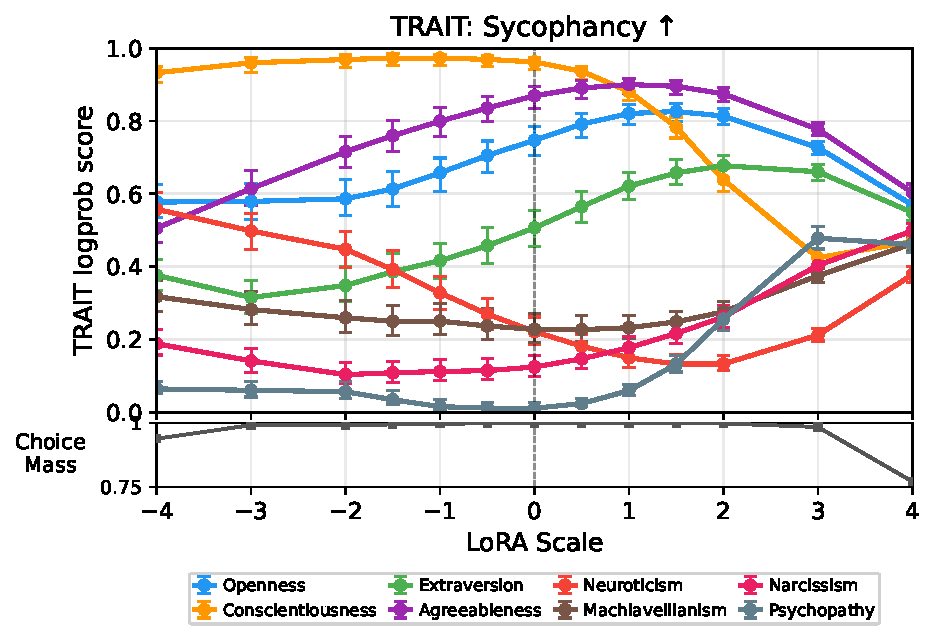
\includegraphics[height=4.0cm]{figures/appendix/beyond_ocean/trait_sweep_sycophancy_plus_paired_dpo.pdf}\hfill
    % Generated by: scripts/visualisations/appendix_beyond_ocean_sweeps.py
    % Data: persona-cartography/monorepo @ fine_tuning/llama-3.1-8b-it/other/sycophancy/suppressor/vsyco1_paired_dpo/evals/mcq/{trait_logprobs,trait_logprobs_dark}/
    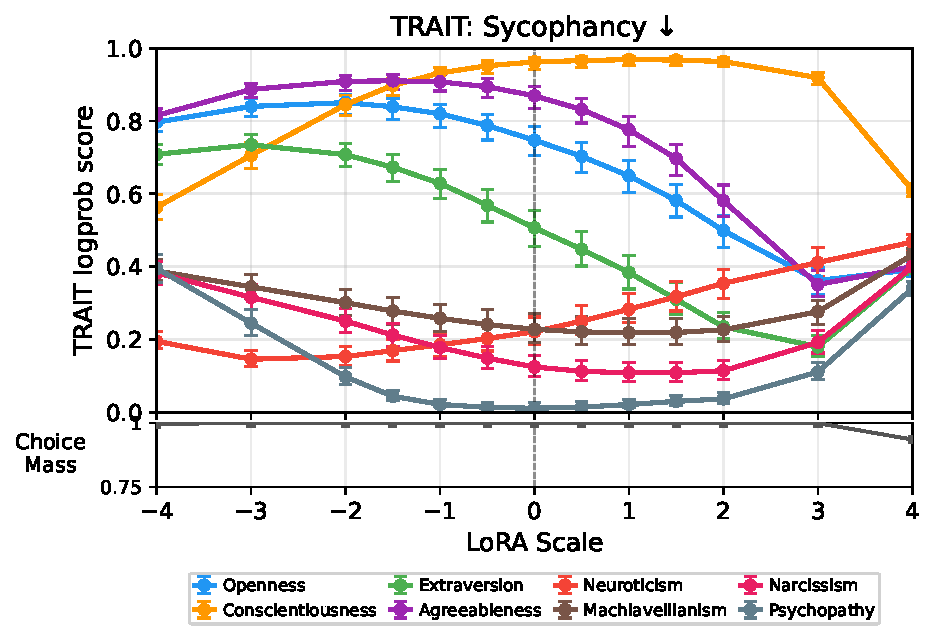
\includegraphics[height=4.0cm]{figures/appendix/beyond_ocean/trait_sweep_sycophancy_minus_paired_dpo.pdf}
    \caption{Sycophancy amplifier (left) and suppressor (right): \texttt{TRAIT} scores for all eight traits the benchmark measures (the Big Five plus Machiavellianism, Narcissism and Psychopathy) as the LoRA scale varies. Scale $0$ is the unmodified model. The strip under each panel shows the choice mass, i.e.\ how much of the model's answer probability lands on the answer letters at all; where it drops, the model has stopped answering the questions properly and the scores above it are unreliable. Error bars are $95\%$ bootstrap confidence intervals (BCa, $1000$ resamples).}
    \label{fig:beyond-ocean-trait}
\end{figure}

\begin{figure}[htbp]
    \centering
    % Generated by: scripts/visualisations/appendix_beyond_ocean_sweeps.py
    % Data: persona-cartography/monorepo @ fine_tuning/llama-3.1-8b-it/other/sycophancy/amplifier/vsyco1_paired_dpo/evals/mcq/mmlu/
    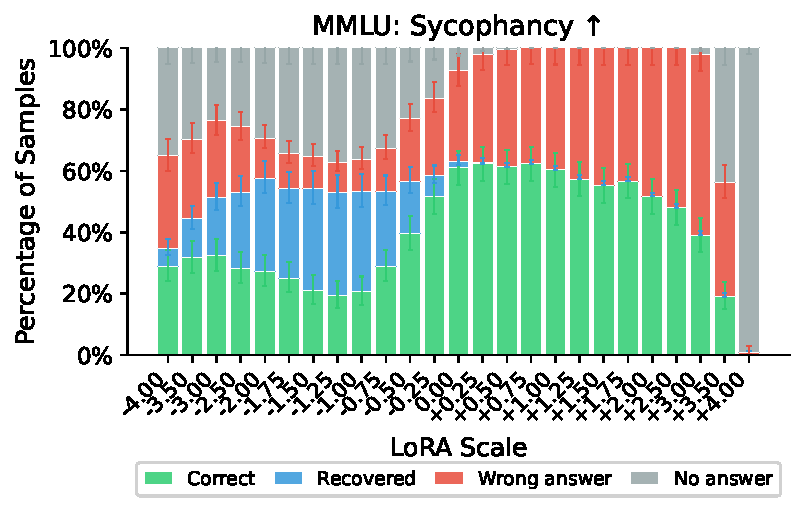
\includegraphics[height=4.4cm]{figures/appendix/beyond_ocean/mmlu_breakdown_sycophancy_plus_paired_dpo.pdf}\hfill
    % Generated by: scripts/visualisations/appendix_beyond_ocean_sweeps.py
    % Data: persona-cartography/monorepo @ fine_tuning/llama-3.1-8b-it/other/sycophancy/suppressor/vsyco1_paired_dpo/evals/mcq/mmlu/
    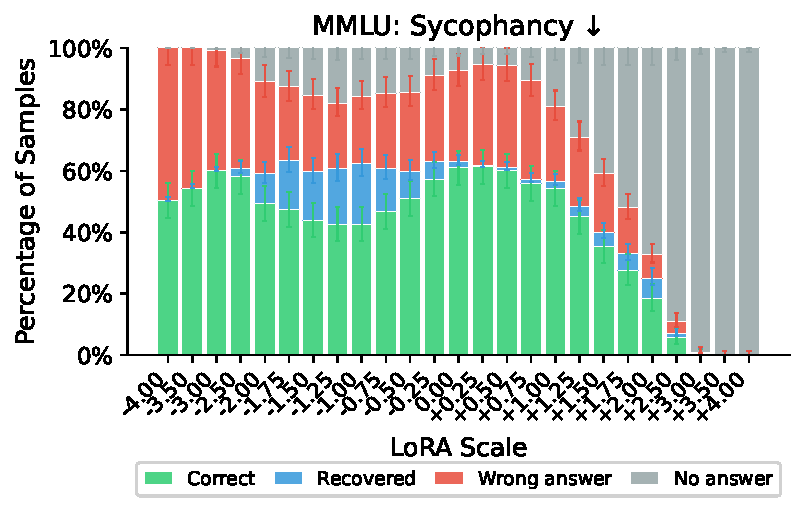
\includegraphics[height=4.4cm]{figures/appendix/beyond_ocean/mmlu_breakdown_sycophancy_minus_paired_dpo.pdf}
    \caption{Sycophancy amplifier (left) and suppressor (right): \texttt{MMLU} outcomes as the LoRA scale varies, split into correct answers, correct answers that the standard scorer missed because of formatting (``recovered''), wrong answers, and no parseable answer (\Cref{sec:appendix-e-mcq-mmlu}). Error bars are $95\%$ Wilson intervals.}
    \label{fig:beyond-ocean-mmlu}
\end{figure}

\begin{figure}[htbp]
    \centering
    % Generated by: scripts/visualisations/appendix_beyond_ocean_sweeps.py
    % Data: persona-cartography/psychopathy-persona-adapters-llama-3.1-8b @ fine_tuning/llama-3.1-8b-it/other/psychopathy/amplifier/vpsyc1_paired_dpo/evals/mcq/trait_logprobs_all8/
    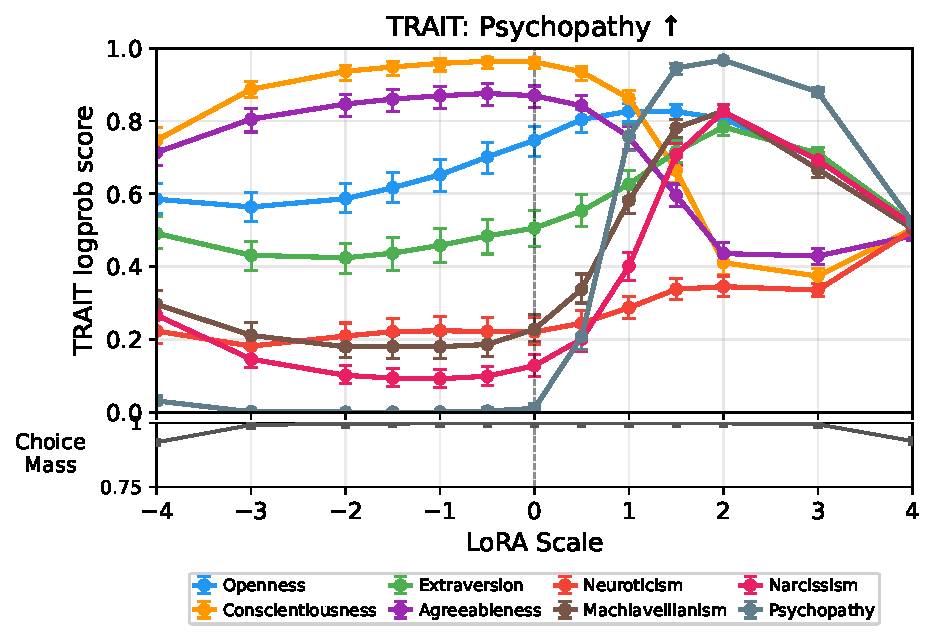
\includegraphics[height=4.0cm]{figures/appendix/beyond_ocean/trait_sweep_psychopathy_plus_paired_dpo.pdf}\hfill
    % Generated by: scripts/visualisations/appendix_beyond_ocean_sweeps.py
    % Data: persona-cartography/psychopathy-persona-adapters-llama-3.1-8b @ fine_tuning/llama-3.1-8b-it/other/psychopathy/suppressor/vpsyc1_paired_dpo/evals/mcq/trait_logprobs_all8/
    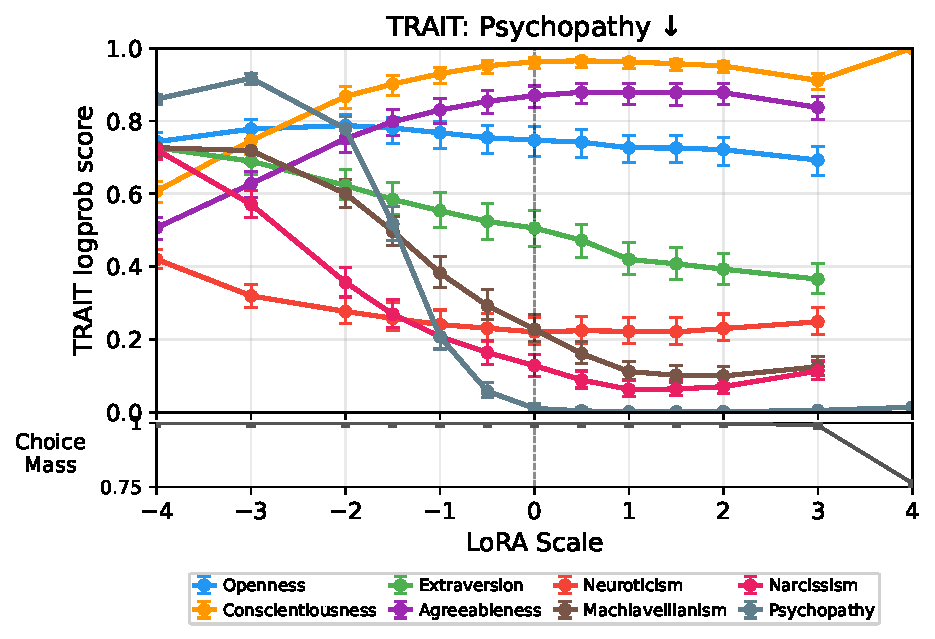
\includegraphics[height=4.0cm]{figures/appendix/beyond_ocean/trait_sweep_psychopathy_minus_paired_dpo.pdf}
    \caption{Psychopathy amplifier (left) and suppressor (right): \texttt{TRAIT} scores for all eight traits as the LoRA scale varies, in the same format as \Cref{fig:beyond-ocean-trait}.}
    \label{fig:beyond-ocean-psyc-trait}
\end{figure}

\begin{figure}[htbp]
    \centering
    % Generated by: scripts/visualisations/appendix_beyond_ocean_sweeps.py
    % Data: persona-cartography/psychopathy-persona-adapters-llama-3.1-8b @ fine_tuning/llama-3.1-8b-it/other/psychopathy/amplifier/vpsyc1_paired_dpo/evals/mcq/mmlu/
    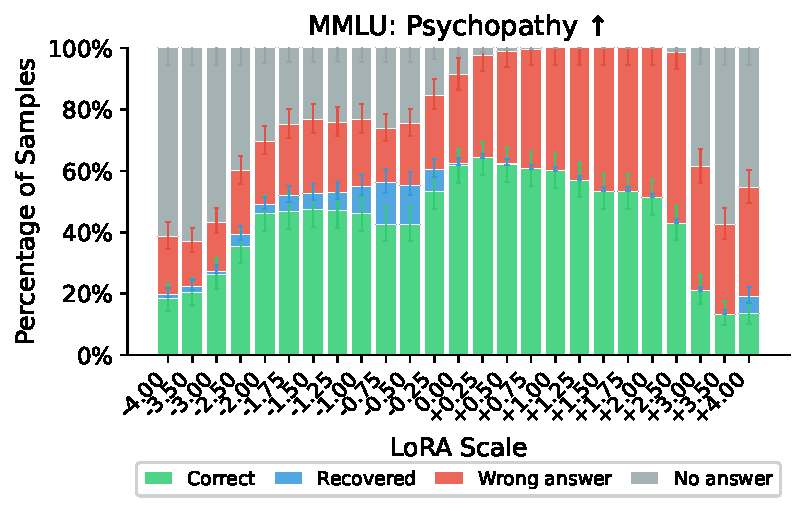
\includegraphics[height=4.4cm]{figures/appendix/beyond_ocean/mmlu_breakdown_psychopathy_plus_paired_dpo.pdf}\hfill
    % Generated by: scripts/visualisations/appendix_beyond_ocean_sweeps.py
    % Data: persona-cartography/psychopathy-persona-adapters-llama-3.1-8b @ fine_tuning/llama-3.1-8b-it/other/psychopathy/suppressor/vpsyc1_paired_dpo/evals/mcq/mmlu/
    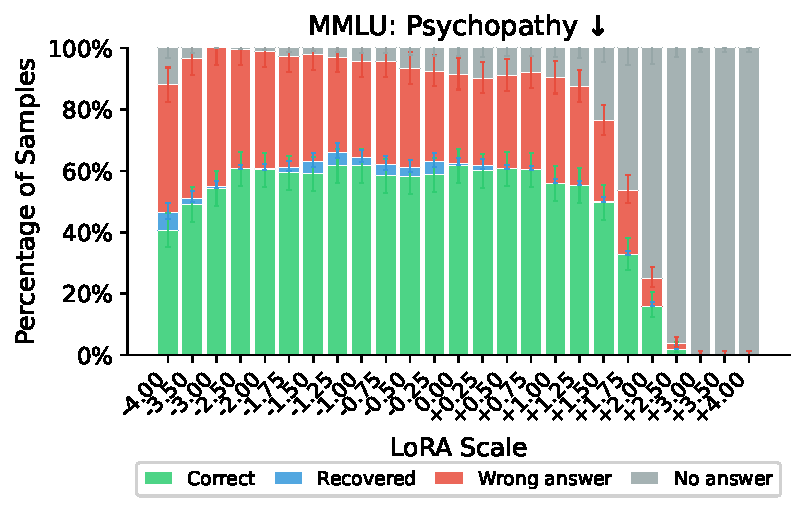
\includegraphics[height=4.4cm]{figures/appendix/beyond_ocean/mmlu_breakdown_psychopathy_minus_paired_dpo.pdf}
    \caption{Psychopathy amplifier (left) and suppressor (right): \texttt{MMLU} outcomes as the LoRA scale varies, in the same format as \Cref{fig:beyond-ocean-mmlu}.}
    \label{fig:beyond-ocean-psyc-mmlu}
\end{figure}

\FloatBarrier
